% This is samplepaper.tex, a sample chapter demonstrating the
% LLNCS macro package for Springer Computer Science proceedings;
% Version 2.20 of 2017/10/04
%
\documentclass[runningheads]{llncs}
%
%\documentclass{ecai}
\usepackage{graphicx}
\usepackage{latexsym}

% Language setting
\usepackage[english]{babel}
% Set page size and margins
%\usepackage[letterpaper,top=2cm,bottom=2cm,left=3cm,right=3cm,marginparwidth=1.75cm]{geometry}
% Useful packages
\usepackage{amsmath}
\usepackage{amssymb}
\usepackage{amsfonts}
%\usepackage{amsthm}
\usepackage{mathrsfs}
\usepackage{graphicx}
%\usepackage[colorlinks=true, allcolors=blue]{hyperref}
% For tree design
\usepackage{fancybox}
\usepackage{tikz}
%\usepackage{parskip}
% For algorithms
\usepackage{algorithm}
\usepackage[noend]{algpseudocode}
% For the appendix
\usepackage[toc,page,title,titletoc,header]{appendix}
%\renewcommand{\appendixpagename}{Annexes}

% For heat map
\usepackage{pgfplotstable}
\pgfplotsset{compat=1.18}

\renewcommand{\floatpagefraction}{.98}%

\pgfplotstableset{
    color cells/.style={
        col sep=comma,
        string type,
        postproc cell content/.code={%
                \pgfkeysalso{@cell content=\rule{0cm}{2.4ex}\cellcolor{black!##1}\pgfmathtruncatemacro\number{##1}\ifnum\number>50\color{white}\fi##1}%
                },
        columns/x/.style={
            column name={},
            postproc cell content/.code={}
        }
    }
}

\DeclareMathOperator{\as}{\text{arg}\sigma}

% Bridge
\newenvironment{cardhand}[0]{
    \newbox\mnord
    \newbox\msud}{
\begin{tabular}{*{2}{c@{\quad\ }}}
NORTH&SOUTH\\[10pt]
\box\mnord&\box\msud
\end{tabular}
}
\newenvironment{cardtable}[0]{
    \newbox\mnord
    \newbox\msud
    \newbox\centre}{
    \setbox\centre=\hbox{
        \begin{tabular}{|lcr|}
            \hline
            &N&\\[10pt]
            &S&\\
            \hline
        \end{tabular}
    }
    \vskip 0.5cm
    \begin{tabular}{ccc}
        &\box\mnord\\
        &\\
        &\box\centre\\
        &\\
        &\box\msud
    \end{tabular}
    \vskip 0.5cm
}

\newenvironment{nord}[0]{\lrbox{\mnord}\tabular{c*{13}{c@{\ }}}}{\endtabular\endlrbox}
\newenvironment{sud}[0]{\lrbox{\msud}\tabular{c*{13}{c@{\ }}}}{\endtabular\endlrbox}
\newcommand\pique[1]{$\spadesuit$&#1\\}
\newcommand\coeur[1]{$\heartsuit$&#1\\}
\newcommand\carreau[1]{$\diamondsuit$&#1\\}
\newcommand\trefle[1]{$\clubsuit$&#1\\}
%\newcommand\suit[1]{$\mathfrak{0}$&#1\\}
%end Bridge

\begin{document}
%
\title{Trick Costs for $\alpha\mu$ and New Relatives
}
%
%\titlerunning{Abbreviated paper title}
% If the paper title is too long for the running head, you can set
% an abbreviated paper title here
%
\author{Samuel Bounan\inst{1} \and
Stefan Edelkamp\inst{2,3}}
%
\authorrunning{F. Author et al.}
% First names are abbreviated in the running head.
% If there are more than two authors, 'et al.' is used.
%
\institute{École normale supérieure de Lyon,
Auvergne-Rhône-Alpes, 
France
\email{samuel.bounan@ens-lyon.fr}
\and
Department of Theoretical Computer Science and Mathematical Logic, 
Faculty of Mathematics and Physics,
Charles University in Prague 
\email{edelkamp@ktiml.mff.cuni.cz}
\and
Computer Science Department,
Faculty of Electrical Engineering,
Czech Technical University in Prague
\email{edelkste@fel.cvut.cz}
}
%
\maketitle              % typeset the header of the contribution
%
\begin{abstract}
In this paper we present a player for incomplete information
card games with tricks scored by points or eyes. We factorize existing algorithms into a template that captures the main ingredients of such game trees. We then analyze three different algorithms, and the impact of the information given during the algorithm on the decisions it makes. We extend these algorithms to work with cost instead of winning vectors, and illustrate their effectiveness in finding good cards. We develop a new algorithm that tries to respect known information.

\keywords{Tree search  \and Game theory \and Card games.}
\end{abstract}
%
%
%
\section{Introduction}

Many perfect-information board games such as Checkers~\cite{checkers}, Oware~\cite{Oware}, Connect4~\cite{connectfour}, Awari~\cite{DBLP:journals/computer/RomeinB03}, and Nine-Men-Morris~\cite{ninemenmorris} have been solved, or, as in Chess, Shogi or Go, computer AIs clearly outperform humans~\cite{alphazero}. 
Therefore, research attention has shifted to incomplete information games. The partially observable board game Stratego
has recently been analyzed with \emph{DeepNash}, a model-free multiagent reinforcement learning algorithm~\cite{Perolat_2022}. It achieved an all-time top-3 rank on the Gravon games platform, competing with human expert players. 

Card games remain an objective of research for decision making with imperfect information. After some variants of Poker have been solved or played to a satisfying degree~\cite{poker,DBLP:journals/corr/MoravcikSBLMBDW17}, trick-taking games such as Skat~\cite{DBLP:conf/ijcai/BuroLFS09,diplomkupfersc}, Hearts~\cite{DBLP:conf/cg/SturtevantW06} and Bridge~\cite{DBLP:journals/corr/abs-1911-07960,frank1998search,ab_generalisation_2022} have been identified as current AI challenges. 
%While self-playing experiments suggest even more elaborated computer play, according to the first Human-AI Skat competition, top humans still played bett,er. 
One obstacle is that, given the large number of tricks and degree of uncertainty, a direct application of reinforcement learning as in Go~\cite{AlphaGo} is less obvious.

Most recently, some card game AIs are beginning to challenge human supre- macy. Notably worldclass caliber play in Bridge~\cite{cazenave_$$alpha$$_2021,DBLP:journals/corr/abs-1911-07960}, Spades~\cite{DBLP:conf/ecai/CohensiusMOS20},
and
Skat~\cite{edelkamp_knowledge-based_2021,hope}. In these 
cutting-edge players, domain-dependent information is provided, such as winning probabilities extracted from human expert games~\cite{edelkamp_challenging_2019}.
We have implemented an efficient framework for general card games. General game playing has a long tradition: there
have been several insightful international competitions using GDL or GDL-II (for incomplete information)~\cite{Schiffel2011a} as the input language. While the players achieved a remarkable playing strength~\cite{finnsson2007cadia}, the generation of moves is  slow. Even faster frameworks like Google DeepMind's \emph{OpenSpiel} are less efficient for card games than our
framework with its concise card encodings.

Another problem is that for multi-player teams most general game playing algorithms are not yet competitive. We focus on trick-taking stage of card 
games. While we have implemented bidding and dog putting strategies for all the card games, they are not the subject of this work, as they are often based on domain-dependent conventions. 

The paper is organized as follows. 
First we will define the building blocks for the formalization of the problem. Our notation is not taken from any specific work, but helps to design a naive algorithm. Section~\ref{minimax} refers 
to the construction of the driver template algorithm. Then, we discuss the efficiency of three algorithms. The first one, called Perfect Information Monte-Carlo, PIMC, is well-known~\cite{GIB}. The second one, $\alpha\mu$ is newer \cite{cazenave_$$alpha$$_2021} and shown effective in Bridge. The third one is a new. In all three, we present the algorithm principles in a template algorithm %\ref{algo:template}, 
thus adapt them to our model. Also, $\alpha\mu$ was only used with Boolean score vectors and with two players. We extend it to scores in $\mathbb{R}$ and to several players. Finally, we present some results we obtained in our implementation. Our code generalizes ideas from \cite{edelkamp_knowledge-based_2021} to implement, while in a restricted setting with simplified bidding. 
%Last but not least, all the points discussed in the annexes are of our contribution.
The contribution of this paper are as follows. We
%\begin{itemize}
%\item 
provide an efficient framework.
%\footnote{In case of acceptance we will release the source code} implementation of general trick-taking card games;
%\item 
calculate the effect of truncating tree search with subsequent random playouts.
%\item 
quantify the information gain of $\alpha\mu$ wrt\ PIMC.
%\item 
successfully apply $\alpha\mu$ algorithm to 
support more players in a team and to general trick costs; 
%\item 
propose a novel general incomplete-information algorithm as a compromise of different nodes in the backup. 
%\item an evaluation in the Game Bridge and Belote and of interactive play against other bots that include more domain-dependent knowledge. 
%\end{itemize}

\section{Preliminaries} \label{section:formalisation}

%While there are many formalizations of games, e.g., in extensive form~\cite{HART199219}, we prefer a pragmatic 
%description.

%\subsection{General Rules for Card Games}

%\begin{definition} %[Cards, Worlds, Game States]
The \emph{set of cards} $\mathcal{C}$ is dealt to $p$ players at the beginning of the game. A \emph{world} is any possible deal of the cards among the players, $\mathcal{W}$ the set of worlds, and for a world $w \in \mathcal{W}$, $w_i$ denotes the hand of player $i$, $i \in \{1,\ldots,p\}$. 
Worlds change during a game.
We call \emph{state} the history of cards already played, and $\mathcal{S}$ the set of possible states.
%\end{definition}

%\begin{definition} [Turn, Termination, Score]
In a state $s$, the \emph{next player} to play a card is determined by a function $\mbox{\em turn}(s) \in \{1,\ldots p\}$ and the set of \emph{legal cards} that can be played in $s$ with a hand $w_i$ by $\mbox{\em legal}(w_i,s) \subseteq \mathcal{C}$. In some states the game ends, this is determined by a Boolean function $\mbox{\em over}(s)$, and in these cases each player receives an amount of points given by a function $\mbox{\em score}(i,s) \in \mathbb{R}$. The goal of each player is to maximize its final score, and we assume rationality of everyone and common knowledge of rationality. 
%\end{definition}
%\begin{definition} [Knowledge]
In general in a state $s \in {\cal S}$ the world is neither perfectly known nor completely unknown and with a hand $w_i$ player $i \in \{0,\ldots,p\}$ assumes a particular distribution on the set of worlds $D_{i,w_i,s}$. 
%\end{definition}

%E.g., in the game of Bridge, there are two teams of two players playing with 52 cards, $\mbox{\em turn}(s)$ is the next player $p \in \{1,\ldots,4\}$ at the table if the current trick is not over, and the winner of the trick, if it is. The legal cards are defined by the rule \emph{if you have the suit, you have to follow}. The winner of a trick is either the highest card of the required suit (the suit of the first card played), if no trump was played, or the highest trump (the increasing order of the cards  $2,3,4,5,6,7,8,9,T,J,Q,K,A$). The game is \emph{over} when 13 tricks have been made, and the \emph{score} of each team's score increases with the number of tricks they made.
%\subsection{Problem Description}
To construct an artificial player, we (only) need to know in a state $s$, in a position $i$ and with a hand $h$,  what is the best card to play. In extension to articles that formalize tree searches, as in \cite{calculating_pimc}, \cite{understanding_pimc} we chose the following definition. 

%\begin{definition}[Best Score]
If we define $\sigma (i, h, s) \in \mathbb{R}$ as the best score that can be obtained, with $\text{arg}\sigma$ to denote a probabilistic function that returns a card corresponding to the maximum score, uniformly chosen in $\mathcal{U}$ among cards that satisfy this property, we have
\begin{equation*}
    \label{formalisation}
     \sigma (i, h, s) = \text{max}_{c \in \mbox{\em legal}(h,s)} \mathbb{E}_{w \hookrightarrow D(i, h, s)} \mathbb{E} _ {f \hookrightarrow \mathcal{U}(\mathcal{F})} \mbox{\em score}(i,f)
\end{equation*}
where $\mathcal{F}$ is the set of possible optimal final states.
With $s_1 = s$ and $s_{k+1} = s_k \cup \text{arg}\sigma (\mbox{\em turn}(s_k), w_{\mbox{\em turn}(s_k)} \setminus s_k, s_k)$
for $k>1$ we have
$$ \mathcal{F} = \{ f \in \mathcal{S} \mid \exists k \in \mathbb{N} \quad \mathbb{P} [s_k = f] \ne 0 \text{ and } \mbox{\em over}(f) \}. $$
%\end{definition}

Every object can be easily derived from the rules, except the knowledge distribution $D_{i,h,s}$.  
We will construct $O$ the set of possible worlds with a non-zero probability for $D$. 

%\begin{definition} [Distribution]
Let $w$ be a world in ${\cal W}$ with state $s$ and hand $h$.  We have the following constraints on $w$: a) $w_i = h$; and b) in every state before $s$, the players played optimally (because of rationality).
Let $n$ be chosen, so that $s$ is an $n$-tuple. Let $s_k$ be the card played in $s$ at step $k < n$. From the second constraint, we know that in the state $s_{|k} = (s_1, \dots s_k)$ player $\mbox{\em turn}(s_{|k})$ played a card $s_{k+1}$ so that $\mathbb{P}[s_k = \as (\mbox{\em turn}(s_{|k}), w_{\mbox{\em turn}(s_{|k})} \setminus s_{|k}, s_{|k})] \ne 0$. We have
\begin{eqnarray*}
O &=& \{ w \in \mathcal{W}; w_i =h \text{ and } \forall k \in [n] \\ 
&& \quad \mathbb{P} [s_{k+1} = \as (\mbox{\em turn}(s_{|k}), w_{s_{|k}} \setminus s_{|k}, s_{|k}] \ne 0. \}
\end{eqnarray*}
Because no additional knowledge can be used to infer a probability among this set of possible worlds $O$ we have $D_{i,h,s} = \mathcal{U}(O)$.
%\end{definition}
%
There are two problems with this definition of $D$. First, in practice players may differ from the perfect rationality, and restricting $O$ to the worlds where everyone played optimally can quickly become a strong bad bias. Second, computing $O$ is computationally costly (it needs to compute $\sigma$ several times). %Hence, we focus on other parts of the algorithm. 
%
To simplify $D_{i, h,s}$ we assume it follows an uniform distribution over the set of \emph{legal} worlds $P$, that can be computed in constant time as $D_{i,h,s} = \mathcal{U}(P)$ with
    $w \in P$ iff $w_i = h$ and 
   for all $k < n$ we have $s_{k+1} \in \mbox{\em lega}l(w_{\mbox{\em turn}(s_{|k})}, s_{|k}).$

%In most games a card is legal if you don't have any other cards. Thus, 
From a card played by a player $i$, as player $j$ can often derive a set of 
cards that player $i$ does not have (initially, player $j$'s hand, maybe enlarged by certainties through the bidding process). We can represent the knowledge of a player $j$ with sets $\neg K^j_i$ corresponding to the cards that player $j$ knows that player $i$ must not have. This ease the exploration and the search tree can be pruned based on the knowledge.
When a card $c$ has been played by player $i$, we can update $\neg K^j_i$ efficiently with Algorithm \ref{update}.
\begin{algorithm}[t]
\caption{$\mbox{\em update}(\neg K^j_i, c, s)$}
\label{update}
\begin{algorithmic}

\For{$c' \in \mathcal{C} \setminus \neg K^j_i$}
\If{$c \notin \mbox{\em legal}(\{c,c'\}, s)$}
 \State $\neg K^j_i \gets \neg K^j_i \cup \{c'\}$
\EndIf 
\EndFor
\end{algorithmic}
\end{algorithm}
With this reduction of $D$ we study the general structure of the algorithm we want to design.


\section{Minimax Truncated with Random Playouts}
\label{annex:playouts}

Most algorithms include a fast open-card solver to compute the game value. There are different approaches but they all use the minimax search tree as their basis. Note that due to the tricks taken and the teams the max or min modes may not alternate on each path.
%
Finding the optimal result of a minimax tree can be computationally expensive, so an intuitive idea is to limit its depth by estimating the score of a node at the maximal depth by random playouts of the end of the game. In our case, the tree is not that deep, and we have more information on the knowledge of the players, starting with the knowledge that each leaf of the tree is at a constant depth. It is, therefore, possible to obtain a bound on the error made by approximating the optimal score with these playouts, in particular by taking the average of the score obtained by a number of random playouts.

%\subsubsection*{Bounds on Playouts}

Suppose we have a perfect alternating minimax tree $T$. Given the outcomes at each leaf of $T$, we know that some of them cannot be the optimal minimax score. Let $s^*$ denote the optimal score. 
%
\begin{figure}[t]
    \centering
    \caption{Depth-1 minimax tree.}
    \label{treke}
    %\vspace{0.5cm}
    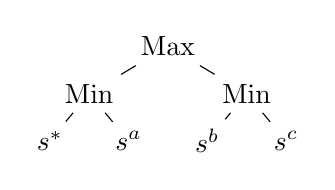
\begin{tikzpicture}[level/.style={sibling distance=50mm/#1},scale=0.4]
    \node (a){Max}
        child {node (b) {Min}
            child {node (d) {$s^*$}}
            child {node (d) {$s^a$}}
        }
        child {node (c) {Min}
            child {node (d) {$s^b$}}
            child {node (d) {$s^c$}}
        };
    \end{tikzpicture}
\end{figure}
%
In Figure~\ref{treke}, we know that $s^a \geq s^*$ because \emph{Min} would otherwise play for $s^a$. We also know that one of $s^b$ and $s^c$ is lower than $s^*$ because \emph{Max} chooses the left subtree in the optimal strategy. So we know that if we order the scores of the leaves $s_1 \leq s_2 \leq s_3 \leq s_4$, we have $s^* \in \{s_2, s_3\}$. More generally, we can compute the number of playouts $g$ (resp. $l$) that have a score higher (resp. lower) than $s^*$.
%
We will estimate the exact number of playouts  greater and less than $s^*$ that are needed to be certain that $s^*$ is optimal for the minimax strategy. Thus, our bounds on the minimax score will be tight. Note that this is also the minimum number of leaves that an algorithm needs to explore to compute $s^*$. 
%, and that $\alpha \beta$ algorithm achieves this minimum complexity with a perfect ordering of the nodes.
%
We study alternating minimax trees. For consistency, we denote by depth of a tree $T$ the number (\emph{Max},\emph{Min}) nodes to a leaf. To estimate $l$ and $g$ we additionally assume that the number of actions at a given depth $d$ is constant, so that $a_d$ denotes the number of possible actions at the root of a tree of depth $d$ for \emph{Max}, and $b_d$ for \emph{Min}.

First, we compute the number of playouts that have a score greater than $s^*$. We note $s (T)$, the optimal minimax score of a tree $T$. We have  $s(T_{\mbox{\em \tiny init}}) = s^*$. To compute the number of playouts with a score greater than $s^*$ we only need the assumption that $s(T_{\mbox{\em \tiny init}}) \geq s^*$. Indeed, if we know that $s (T) \geq s^*$, it means that \emph{Max} chooses a card $a$ such that for all possible choices $b$ of \emph{Min}, the score of the subtree of $T$ after playing $a$ and $b$ has a score greater than $s^*$. Otherwise \emph{Min} could choose an action that leads to a score that is strictly lower than $s^*$. It follows that $s (T) < s^*$, a contradion. Thus, we have $\exists a ~ \forall b \quad s (T_{a,b}) \geq s^*.$ 

We use the assumptions $s (T_{a,b}) \geq s^*$ to setup a recursion. The terminal case is when $T$ has one node, in which case we have one playout that we know has a score greater than $s^*$. With the above assertion we can deduce that the number of playouts in a tree that have a score greater than $s^*$ depends only on the number of actions \emph{Min} that can made at each node of the tree.
Here, we have made the assumption that in a tree with depth $d$, the number of possible actions for \emph{Min} is a fixed number $b_d$. Thus the number of playouts that achieve a score greater than $s^*$ only depends on the depth of the tree. We can, therefore, define it as a sequence $g_d$. The number $g_d$ represents the number of playouts that have a score greater than the optimal minimax score for a tree of depth $d$. Following what we established earlier, we have  $g_0 = 1$ and $g_d = b_d ~ g_{d-1}$ for all $d >0$.
Finally, we get $g_d = \prod^{d}_{i=1}b_i$.
Symmetrically, we can compute the number of playouts that achieve a score lower than $s^*$ as $l_d = \prod^{d}_{i=1}a_i$.
Assuming $T$ is a perfect alternating minimax tree of depth $d$, the optimal score can be achieved by a playout that is neither among the $l_d -1$ lowest playout scores nor in the $g_d -1$ higher playout scores. So the total number of playouts is $l_d~g_d$.

%\subsubsection*{Bounds on the score}

For a bound on the actual score we need to model the distribution of the playout scores. We assume that the number of points that can be won in $T_d$ is
$ S_d$ (we assume here that the minimum score that can be obtained is $0$ but we can easily adjust the result with $S_d$ in $s_{\mbox{\em \tiny max}}(T_d) - s_{\mbox{\em \tiny min}}(T_d) $). We will, therefore, model the distribution of score with a binomial law of parameters $n = S_d$, $p$ unknown. We approximate this law by $\mathcal{N}(\mu,\,\sigma^{2})$ with $\mu = S_dp$ and $\sigma = \sqrt{S_dp(1-p)}$. In this setting we can compute bounds on $s^*$ directly. In fact, a lower bound on $s^*$ is given by the value of the ${l_d}/(l_d~g_d)$ quantile, as we showed above. We have
$Q({l_d}/(l_d~g_d)) \leq s^* \leq Q((l_d~g_d-g_d)/(l_d~g_d))$
with $Q$ being the quantile function of the normal distribution
$Q(p) = \mu + \sigma \sqrt{2}~f^{-1}(2p-1)$
and $f$ being shorthand for $\emph{erf}$. 
By estimating $s^*$ as the midpoint between the two quantiles ($\mu$ in our model) we can estimate the error $\epsilon_d$. For simplicity we assume that $g_d = l_d = n_d \geq 2$ (symm. \emph{Min} / \emph{Max}). Thus, we have ${l_d}/(l_d~g_d) = 1/{n_d} $, so that the error is:	
\begin{align*}
	\epsilon_d =& \frac{Q\big(\frac{n_d-1}{n_d}\big) - Q\big(\frac1{n_d}\big)}{2} \\
							&= \frac{\sigma \sqrt{2}~\big(f^{-1}(1-\frac2{n_d})-f^{-1}(\frac2{n_d}-1)\big)}{2} & \\
							&= \frac{\sigma}{\sqrt{2}}\bigg(2 \cdot f^{-1}\big(1-\frac2{n_d} \big)\bigg)  \ \ \mbox{(symmetry of  $f^{-1}$)} 
\end{align*}

We set
\noindent$\sigma = \sqrt{S_dp(p-1)} \leq \frac{\sqrt {S_d}}{2},$
so that
$\epsilon_d \leq \sqrt{\frac {S_d}2} ~ f^{-1}\big(1-\frac2{n_d}\big).$

%\subsubsection{Approximation of $s^*$}

If we approximate $s^*$ with the mean of the score obtained by a number $m$ of random playouts $\hat{\mu}$, we have, using the Bienaymé-Tchebychev inequality for the normal approximation
$P(|\hat{\mu} - \mu| \geq \epsilon_m) \leq \frac{\sigma^2}{m\epsilon_m^2} = \frac {S_d}{4m\epsilon_m^2}.$
Adding the estimation error, we know that by choosing 
$m \geq \frac{S_d}{4\delta \epsilon_m^2}$ we have 
$P(|\hat{\mu} - s^*| \geq \epsilon_m + \epsilon_d) \leq \delta.$

%\subsubsection{Application in Belote}

For Belote we set $n_d = 2^d d!$ and $S_d = 10d$. % and get
%and obtain
%\begin{align*}
% \epsilon_2 = 1.58 \quad & 1\% \quad &\text{(trick 8)} %\\
% \epsilon_4 = 8.68 \quad & 5\% \quad  &\text{(trick 7)} %\\
%\epsilon_6 = 15.82 \quad & 10\% \quad &\text{(trick 6)} %\\
% \epsilon_8&= 25.29 \quad & 16\% \quad &\text{(trick 5)} 
%\end{align*}
%
%Thus, 
if we want a $20$\%-approximation of the score, valid with a $95\%$ chance, we can estimate the tree after the $5^{th}$ trick, with $m = 8$. If we want to have a $15\%$-approximation valid with a $95\%$ chance, we can cut after the $6^{th}$ trick with $m = 3$.


\section{Template Algorithm}
\label{minimax}



Following $\sigma(i,a,s)$ %(\ref{formalisation}) 
we design a first naive Algorithm \ref{algo:naive} to solve our problem, which branches on every maximum and expectation of $\sigma$.  
The problem with this algorithm is its time complexity. Let $T(d)$ denote the time complexity of the algorithm if $d$ cards are still to be played before the game is over. We have 
$T(d) = |\mbox{\em legal}(h,s)| \cdot |P| \cdot T(d-1)$.
If we assume (for the sake of clarity) the number of legal cards to be fixed during the game, and that the number of possible worlds to be constant, we have $T(d) = K^d$, where $K$ is a constant. Because of this time complexity the naive algorithm is not practical. 
%
\begin{algorithm}[t]
\caption{$\mbox{\em naive}$}
\label{algo:naive}
\begin{algorithmic}
\Function{$\mbox{\em search}$}{$i$, $h$, $s$}
    \State $\mbox{\em res} \gets \{s\}$
    \State $\mbox{\em max} \gets \bot$
    \For{$c \in \mbox{\em legal}(h,s)$}
        \State $j \gets \mbox{\em turn}((s,c))$
        \State $\mbox{\em score}' \gets \bot$
        \For{$w \in P$}
            \State $F \gets \mbox{\em search}(j, w_j, (s,c))$
            \For{$x \in F$}
                \State $\mbox{\em score}' += \mbox{\em score}(i,x) / |F \times P|$
            \EndFor
        \EndFor
        \If {$\mbox{\em score} > \mbox{\em max}$}
        	\State $\mbox{\em res} \gets \{ c \}$
        	\State $\mbox{\em max} \gets \mbox{\em score}'$
        \ElsIf{$\mbox{\em score}' = \mbox{\em max}$}
        	\State $\mbox{\em res} \gets \mbox{\em res} \cup \{c\}$
        \EndIf
    \EndFor
    \State \Return \mbox{\em res}
\EndFunction
\\
\Function{$\mbox{\em chooseCard}$}{$h$, $s$}
%    \State $S \gets {\bf 0} \in \mathbb{R}^{|\mbox{\em \tiny legal}(h,s)|}$
    \For{$c \in \mbox{\em legal}(h,s)$}
        \State $F \gets \mbox{\em search}(\mbox{\em id}, h, s)$
        \State $S[c] \gets \mu_{f \in F}(\mbox{\em score}(\mbox{\em id}, f))$
    \EndFor
    \State \Return $\arg \max S$
\EndFunction
        
\end{algorithmic}
\end{algorithm}
%
The common methods to solve this problem use the same set of worlds for all nodes in the search tree. This was not the case in our naive algorithm, where each node branches to its possible set of worlds $P$. Let us assume a set of worlds $W$ for whole tree. We will give each node a value representing the optimal scores in state $s$ for the worlds in $W$. The type of value depends on the specification of the algorithm, it will be some kind of array indexed by $w \in W$ with the optimal scores of each $w$. It should contain the scores of each player, as it will be the only value passed through the tree.

With this tree, it is often easy to cut some unused nodes using deep pruning, as in the $\alpha\beta$ pruning algorithm. %ref{algo:ab}. 
This pruning is essential in the minimax tree. As shown in \cite{knuth_analysis_1975} we can hope to reach a complexity close to $K^{d/2}$. This is adapted to two player minimax games, with perfect information. It has been extended to other frameworks, for example with \cite{ab_generalisation_2022} to partially ordered values with a cache. We will propose here a new generalization, not very sophisticated, but flexible to different specifications.

%\begin{algorithm}
%\caption{$\alpha\beta(s,\alpha,\beta)$}
%\label{algo:ab}
%\begin{algorithmic}
%\If{$\mbox{\em over}(s)$}
%    \State $ \text{return } \mbox{\em score}(s)$
%\ElsIf{Min team}
%    \State $v \gets +\infty$
%    \For{$s'$ succ of $s$}
%        \State $v \gets \min(v, \alpha\beta(s', \alpha, \beta))$
%        \If{$\alpha \geq v$}
%            \State $ \text{return } v$
%        \EndIf
%        \State $\beta \gets \min(\beta, v)$
%    \EndFor
%\Else
%    \State $v \gets -\infty$
%    \For{$s'$ succ of $s$}
%        \State $v \gets \max(v, \alpha\beta(s', \alpha, \beta))$
%        \If{$\beta \leq v$}
%            \State $ \text{return } v$
%        \EndIf
%        \State $\alpha \gets \max(\beta, v)$
%    \EndFor
%\EndIf
%\State $ \text{return } v$
%\end{algorithmic}
%\end{algorithm}



\section{Imperfect Information Tree Search}
\label{iminimax}


Algorithm~\ref{algo:template} captures the structure of a MiniMax tree search algorithm with vector $\alpha$ and set of worlds $W$.  
%
\begin{algorithm}[t]
\caption{tree}
\label{algo:template}
\begin{algorithmic}

\Function{$\mbox{\em tree}$}{$s$, $\alpha$, $W$, $\mbox{\em parent}$}
    \State $\mbox{\em parent}[\mbox{\em myteam}] \gets \mbox{\em myid}$
    \State $r \gets \mbox{\em init}_{\mbox{\em \tiny myid}}(s, W)$
    \For{$c \in \bigcup_{w \in W} \mbox{\em legal}(s, w_{\mbox{\em \tiny myid}})$}
        \State $\alpha[\mbox{\em myteam}] \gets \max_{\mbox{\em \tiny myid}}(r,\alpha[\mbox{\em myteam}])$
        \If{$\exists t \ne \mbox{\em myteam}: \alpha[t] <_{\mbox{\em \tiny parent}[t]} r$}
            \State $\text{return } \bot_{t}$
        \EndIf
        \State $W_c \gets \{ w \in W \mid c \in \mbox{\em legal}(s, w_{\mbox{\em \tiny myid}}) \}$
        \State $v \gets \mbox{\em tree}(\alpha, (s, c), W_c, \mbox{\em parent})$
        \If{$v = \bot_t$}
            \If{$t \ne \mbox{\em team}$}
                \State \Return $\bot_t$
            \EndIf
        \Else
            \State $r \gets \max_{\mbox{\em \tiny myid}}(r,v)$
        \EndIf
    \EndFor
    \State \Return $r$
\EndFunction
\\
\Function{$\mbox{\em chooseCard}$}{$s$, $h$}
    \State $W \gets \mbox{\em genWorlds}()$
    \For{every team $t$}
        \State $\mbox{\em parent}[t] \gets \emptyset$
        \State $\alpha[t] \gets \bot_t$
    \EndFor
    \State \Return $\arg \mbox{\em criterion}_{c \in \mbox{\em \tiny legal}(s, h)} (\mbox{\em tree}((s,c), \alpha, W, \mbox{\em parent}))$
\EndFunction

\end{algorithmic}
\end{algorithm}
We have
\begin{itemize}
    \item $<_i$ partial order on the pruning preferences of player~$i$;
    \item $init_i(s,W)$, initialize the result for a player $i$, which has to be a lower bound on the actual value (depending on the worlds in $W$) of the node $s$ for $<_i$
    \item $\max_i$ calculates the return value based on the values of the children. It is actually a fusion of the values of the children rather than a maximum over $<_i$. %It should return the correct value of a node $s$ constructed from the values of its children
    \item $\mbox{\em genWorlds}()$ generates the worlds over which to compute the values, uses the distribution $D$ of the players.
    %to generate according to the knowledge. %It could be simply the evaluation of $D$ many times, to create a pool of worlds following the law of $D$, but we will need to have some more sophisticated specification for our last algorithm
    \item $\mbox{\em criterion}_i$ a total order representing the preferences of player $i$ for the final choice of the card to play
\end{itemize}

The complexity of this algorithm is hard to study, the partial order causing pruning is difficult to approach and it makes the model deviating from the ones developed in \cite{knuth_analysis_1975}. In practice, however, we can see a significant improvement of time complexity with this pruning.
%
Now that we have a generic algorithm for solving the problem, with an a priori reasonable time complexity, we will compare different specifications of this algorithm.

%\section{Specifications of the template}

%\label{section:specification}

We will explore different specifications of the template we presented. Each one is specified for two teams. The score of a final state is the score made by the \emph{Max} (declarer) team. We tried to adapt it to multiple teams following the work of \cite{multi-pruning}, but it is a long time work. This could probably be done in a future work. The first one is a direct extension of the usual $\alpha \beta$ pruning algorithm for perfect information games. The second one is the one proposed in \cite{cazenave_$$alpha$$_2021}. The last one is a novel contribution. 
In each case we will present the specifications of the functions we have previously invoked. We will not describe the function $\mbox{\em init}_i$ in detail, because we only found a trivial lower bound over the value of a node, based on the score already made by a team in our trick-taking card games.



\paragraph{Perfect-Information Monte Carlo}

The idea of the Perfect-Information Monte Carlo (PIMC) algorithm is to generate random worlds according to $D$, and then  to compute a score in each world \emph{as if it were in perfect information} using the $\alpha\beta$ algorithm. 
The generation of the worlds follows directly from $D$. We generate 
a set of $N$ worlds.
Over the worlds in $W$, the \emph{value} of a node is the score of each world in this setting of perfect information for everyone: $\mathbb{R}^N $. This hypothesis of perfect information in these worlds is not consistent with the settings. To illustrate it, this algorithm fits a game where everyone shows their hand, and plays openly after one card is played. Thus the generation of the worlds tries to capture the initial unknown, and then in each world, we play with perfect information.
Let us talk about pruning. For the \emph{Max} team a value $a$ is greater than $b$ if the score of each world $w \in W$ is greater in $a$ than in $b$:
$ \forall k \in [N] a_k \geq b_k $
It is symmetric for \emph{Min} nodes:
$ \forall k \in [N] a_k \leq b_k $ 
In this framework, we can derive the other function. The function $max_i(a,b)$ returns the maximum/minimum, according to the team of $i$, of each score of $W$. In fact with perfect information the players can choose the "objective" best card in each world. To make the final choice for the card to play, we set the criterion to prefer the best mean of the score, according to the team. The details are presented in Algorithm \ref{algo:pimcam} (left).

\newlength\myindent
\setlength\myindent{-2em}
\newcommand\bindent{%
  \begingroup
  \setlength{\itemindent}{\myindent}
  \addtolength{\algorithmicindent}{\myindent}
}
\newcommand\eindent{\endgroup}
%\addtolength{\algorithmicindent}{\myindent}

\begin{algorithm}[t]
\caption{PIMC (left) and $\alpha\mu$ (right)}
\label{algo:pimcam}
\hspace{-0.5cm}
\begin{minipage}{4.2cm}
\begin{algorithmic}
\Function{$\mbox{\em genWorlds}$}{} 
    \State $W \gets \emptyset$
    \For{$k \in [N]$}
        \State $w \hookrightarrow D$
        \State $W \gets W \cup \{w\}$
    \EndFor
    \State \Return $W$
\EndFunction
\\
\Function{$\mbox{\em max}_i$}{$a$, $b$}
%    \State $r \in \mathcal{V}$
    \For{$k \in [N]$}
        \If{Max team}
            \State \hskip-1.0em $r_k \gets \max(a_i, b_i)$
        \Else
            \State \hskip-1.0em $r_k \gets \min(a_i, b_i)$
        \EndIf
    \EndFor
    \State \Return r
\EndFunction
\\
\Function{$\mbox{\em criterion}_i$}{$a$, $b$}
    \State \hskip-1.0em $s_a \gets \sum_{k=1}^n a_k$
    \State \hskip-1.0em  $s_b \gets \sum_{k=1}^n b_k$
    \If{Max team}
        \State \Return $s_a > s_b$
    \Else
        \State \Return $s_a < s_b$
    \EndIf
\EndFunction
\\
\\
\\
\\
\\
\\
\\
\end{algorithmic}
%\end{algorithm}
\end{minipage} 
\hspace{-0.75cm}
\begin{minipage}{5.25cm}
%\begin{algorithm}
%{\bf $\alpha\mu$}
%\label{algo:am}
\begin{algorithmic} 
\Function{$\mbox{\em max}_i$}{$X$, $Y$}
    \State $R \gets \emptyset$
    \If{root}
        \State $R \gets X \cup Y$
    \Else
        \For{$(x,y) \in X \times Y$}
            \State $r \in \mathbb{R}^N$
            \For{$k \in [N]$}
                \If{Max team}
                    \State \hskip-1em $r_k \gets \max(x_i, y_i)$
                \Else
                    \State \hskip-1em $r_k \gets \min(x_i, y_i)$
                \EndIf
            \EndFor
            \State $R \gets R \cup \{r\}$
        \EndFor
    \EndIf
    \For{$r_1 \ne r_2 \in R$}
        \If{$\forall k \in [N] r_{1k} \leq r_{2k}$}
            \If{root is Max}
                \State remove $r_1$ from $R$
            \Else
                \State remove $r_2$ from $R$
            \EndIf
        \EndIf
    \EndFor
    \State \Return R
\EndFunction
\\
\Function{$\mbox{\em criterion}_i$}{$X$, $Y$}
    \If{Max team}
        \State \hskip-1.0em  $s_X \gets \max_{x \in X}\sum_{k=1}^n x_k$
        \State \hskip-1.0em  $s_Y \gets \max_{y \in Y}\sum_{k =1}^n y_k$
        \State \Return $s_X > s_Y$
    \Else
        \State \hskip-1.0em $s_X \gets \max_{x \in X}\sum_{k=1}^n x_k$
        \State \hskip-1.0em $s_Y \gets \max_{y \in Y}\sum_{k=1}^n y_k$
        \State \Return $s_X < s_Y$
    \EndIf
\EndFunction
\end{algorithmic}
\end{minipage}
\end{algorithm}

\paragraph{$\alpha \mu$ Algorithm}

The problem with PIMC is that it assumes perfect information for everyone. It leads to several imperfections and difficulties in 
decision-making as shown in \cite{frank1998search}. 
An example of a situation where PIMC fails is shown in Fig. \ref{fig:lim_pimc}
(left).
%
South's expected score 
over these two tricks is $0.5$. In fact, South has a $50\%$ chance of discarding the useless ace on the $\clubsuit A$ and keeping the useful ace. In this case South scores $1$, otherwise $0$. However PIMC would generate several worlds, some with North having the $\spadesuit 2$, some with North having the $\heartsuit 2$, and in each one South would score $1$. In fact, if South knows the North's remaining card (this is the case in the PIMC algorithm, where perfect information is given), it is easy to keep the right ace, and to win the last trick. Thus PIMC would average the score over the world sample and predict score $1$ for South, which is a mistake. 

\begin{figure}[t]
\begin{minipage}{4cm}
    \begin{cardtable}
\begin{sud}
\pique{A}
\coeur{A}
\end{sud}

\begin{nord}
\trefle{A} 
${2 \spadesuit | 2 \heartsuit}$
\end{nord}

\end{cardtable}
\end{minipage}
\begin{minipage}{4cm}

    \centering
    \begin{cardtable}

\begin{nord}
\pique{A}
\coeur{A}
\end{nord}

\begin{sud}
\trefle{$\mathbf{A}$}
\pique{(2)}
\end{sud}

\end{cardtable}
\end{minipage}
    \caption{In this game we follow the rules of Bridge except we only play with two enemy players. Trump is clubs. (left) North plays $\clubsuit A$ and South is to play. South does not know if the second card of North is $\spadesuit 2$ or $\heartsuit 2$, it is a $50\%-50\%$ situation. (right) Trump is clubs. North does not know if the second card of South is $\spadesuit 2$ or $\heartsuit 2$. South has to play.}
    \label{fig:lim_pimc}
\end{figure}



The idea with the $\alpha\mu$ algorithm presented in \cite{cazenave_$$alpha$$_2021} is to include the imperfect information of the player who has to choose a card in the reasoning. The player at the root of the tree doesn't know which world is the good one, but the others do and play with perfect information. The algorithm fits a game where one player has to play a card, but everyone else sees his/her hand. Although it is not perfect in terms of the information given, it is an improvement over PIMC. 

We study it using information theory.
Suppose $C$ cards are remaining and player $i$ knows the location of $|C|-k$ of those $C$ cards, $k$ being unknown. We will model $D$ as the uniform distribution on the unknown cards over all players. These unknown cards can be dealt $p^k$ different times. Thus, for $w \in \mathcal{W}$ we have
$D(w) = 1/{p^k}$ (with $p$ the number of players) if $w$ matches the known cards, and $0$, otherwise.

Knowing that we are playing in a world $w^*$ (which is coherent with the known cards of $i$) gives the information $-\log(D(w^*)) = k\log p$. Note that this is also the KL-divergence between the certain distribution where $w*$ has a probability of $1$ and $D$. 
We next measure the total information $I(n)$ given to the players when $n$ cards are to be played. Consider that $n$ cards are unknown at this state, and all the other $C-n$ cards are known.
For a solution given by PIMC we compute the information gain contained in this solution. In Formula~(\ref{formalisation}) every call of $\sigma$ adds some information to this gain: the perfect information given to the node of the state. We have
\begin{align*}
    I_{pimc}(n) &= n \log p + \sum_{k=0}^{n-1} I(k)
    = n\log p + \sum_{k=0}^{n-1} (n-k) k \log p \\
%    &= \log p (n + \sum_{k=0}^{n-1} k(n-k)) \\
    &= \log p (n + {n(n^2 - 1)}/6) \geq \log p ( n^3/6 )
\end{align*}

Now consider a solution of $\alpha\mu$. Perfect information is only given to the non-root player. So, assuming we start with the root. we have

\begin{align*}
    I_{\alpha\mu}(n) &= 0 + \sum_{k=0}^{n-1} (n-k) \delta_{p_{depth=k}, root}(k \log p) \\
    &= \log p \bigg( \sum_{k=0}^{n} (n-k) k - \sum_{i=0}^{n/p} (n-ip) ip \bigg) \\
    &= \log p \bigg(\frac{n(n^2-1)}6 - p^2\frac{\frac{n}{p}((\frac{n}{p})^2-1)}6 \bigg) \\
    &= \log p \bigg( \frac{n^3}6 \bigg) \bigg( 1 - \frac1p + \frac{p-1}{n^2}\bigg).
\end{align*}
Since the expression $\frac{p-1}{n^2}$ is small when we are not at the end of the game (in Bridge in middle game with $7$ tricks left, we have $p=4$, $n=4 \cdot 7$), the information saved with $\alpha\mu$ is about a factor $(1 - 1/p)$. We noticed that with $\alpha\mu$ we achieve a reduction of the information gain by a factor $(1 - 1/p)$. This is not surprising, since we have removed the  
information gift of one player. 

Let us introduce the functions used in $\alpha\mu$. 
This algorithm solves the problem of Fig. \ref{fig:lim_pimc} (left). In 
Fig.~\ref{tree:am} we see that the uncertainty about the outcome of the game is preserved. The value computed, $[(0,1),(1,0)]$ represents the fact that one strategy leads to a nonzero score in one world, and another strategy leads to a nonzero score in the other world.
%
\begin{figure}[t]
    %\centering
    \caption{Application of Fusion algorithm to the problem raised in Fig. \ref{fig:lim_pimc} (left). The scores are the ones of South, viewed as a Max node. Max nodes are circled by continuous line, and Min nodes by dashed lines. Here world 1 is the world where North has $\spadesuit 2$ (the real world), and world 2 is the one where she has $\heartsuit 2$ (the fake world but South doesn't know it).}
    \label{tree:am}
    \hspace{-0.5cm}
    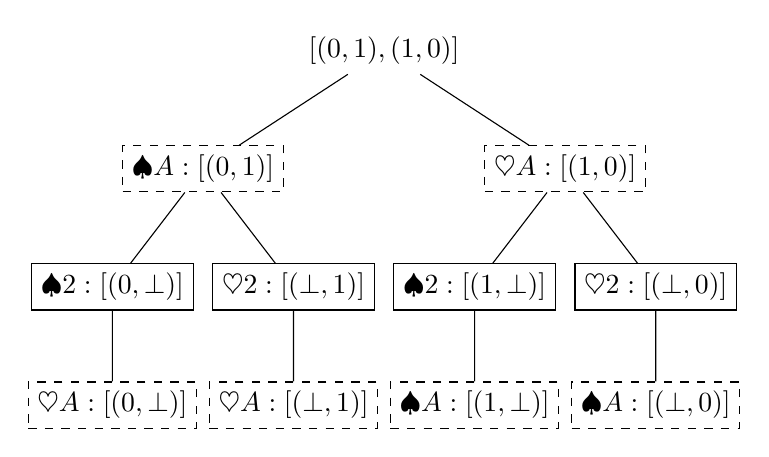
\begin{tikzpicture}[level/.style={sibling distance=46mm/#1}]
    \node {$[(0,1),(1,0)]$}
        child {node [draw, dashed]  {$\spadesuit A: [(0,1)]$}
            child {node [draw] {$\spadesuit 2: [(0,\bot)]$}
                child {node [draw, dashed] {$\heartsuit A: [(0, \bot)]$}}}
            child {node [draw] {$\heartsuit 2: [(\bot,1)]$}
                child {node [draw, dashed] {$\heartsuit A: [(\bot,1)]$}}}}
        child {node [draw, dashed]  {$\heartsuit A: [(1,0)]$}
            child {node [draw] {$\spadesuit 2: [(1,\bot)]$}
                child {node [draw, dashed] {$\spadesuit A: [(1, \bot)]$}}}
            child {node [draw] {$\heartsuit 2: [(\bot,0)]$}
                child {node [draw, dashed] {$\spadesuit A: [(\bot,0)]$}}}}
    ;
    \end{tikzpicture}
\end{figure}

In $\alpha\mu$ $\mbox{\em generateWorlds}$ is the same as in PIMC; $\max_{\mbox{\em \tiny root}}$ computes the union of the values of the children, and removes the elements that are dominated (i.e., if the scores associated with one strategy are all better than another, it removes the latter); $max_i$ is the union of the product of the strategies of the children. One element is computed by taking an element from all the children (we construct one possible strategy for root), and by taking in each world the best score for $i$, as in PIMC (if root follows the constructed strategy, then the score would be the one computed, with perfect information of $i$). Again, the set is simplified by removing the dominated elements for $root$; $criterion$ selects the node containing the strategy with the best expected score over the different worlds in~$W$.


\subsection{Fusion Algorithm}

Even with $\alpha\mu$ we are giving away too much information to the players other than root. This can lead to bugs like the one shown in Fig. \ref{fig:lim_pimc} (right).
%\begin{figure}
%    \label{fig:lim_am}
%\end{figure}
If South plays $\spadesuit 2$, s/he will score $1$. If s/he plays $\clubsuit A$ s/he has $50\%$ chance of scoring $2$ and $50\%$ chance of scoring $1$. So $\clubsuit A$ is the better choice. $\alpha\mu$ supposes perfect information of North. Thus if South plays $\clubsuit A$ she will score $1$, and if s/he plays $\spadesuit 2$ s/he will also score $1$. Both cards are equal, and $\alpha\mu$ could make the mistake of choosing $\spadesuit 2$. 

To solve this problem, we need to incorporate the imperfect information of all the players into our algorithm. This is the goal of the fusion algorithm.
We choose to fix the value of a node to be the expected score of each world if everyone plays optimally according to their knowledge. At a node with two children, player $i$ will choose the value of the child that has the best expectation, according to his/her team, over the worlds that are possible according to his/her knowledge. If the two children have the same expected value, player $i$ has $50\%$ chance of playing each one or them. So the value of the node should be a mixture of both (the middle of the score segment). 

For example, if a Max node has two children $[2,5,3]$ and $[3,7,0]$, its value would be $[2.5,6,1.5]$
The problem with this simple idea is that different players have different knowledge, and different possible worlds. So each set of possible worlds $P$ is different for each player. Moreover for a player, his/her set of possible worlds depends on its hand, that is unknown. We can't take one set $W$ for the whole tree and assume it represents all the players, as we did before. 

We compute the values over subsets of $W$ that correspond to the different $P$ possible for a player. For example, if both  $\emph{Max}$ and $\emph{Min}$ can have two hands, there are four possible worlds $\{\mbox{\em Max}_1\mbox{\em Min}_1, \mbox{\em Max}_1\mbox{\em Min}_2, \mbox{\em Max}_2\mbox{\em Min}_1, \mbox{\em Max}_2\mbox{\em Min}_2\}$. Suppose $\mbox{\em Max}$ is the root, and you want to merge two values at a $\mbox{\em Min}$ node: $[0,2,3,1]$ and $[2,0,2,3]$. If $\mbox{\em Min}$ has hand $1$, the worlds she will consider are the first and third (you do not know the hand of $\mbox{\em Max}$. So the first value is better because it has an expected score of $1.5$ instead of $2$. But if $\mbox{\em Min}$ has hand $2$ the two values have the same expected score over worlds 2 and 4, which is $1.5$. Thus $\emph{Min}$ has a $50\%$ chance of playing each value and we mix the scores of these worlds. We come up with the value $[0,1,3,2]$. A more detailed example is shown in Fig.~\ref{fusion_perm}.
%
\begin{figure}[t]
    \centering
    \caption{Fusion of two values by a Max node. The row correspond to the different hands possible for Min, and the columns the one for Max ($m_{ij}$ represents the score of the world where Min has hand $i$ and Max hand $j$).}
    \label{fusion_perm}
    \vspace{0.5cm} 
    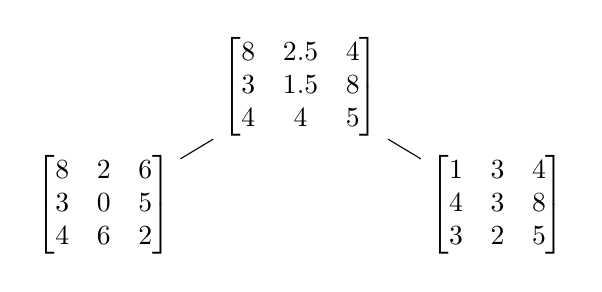
\begin{tikzpicture}[level/.style={sibling distance=50mm/#1}]
    \node (a){$
    \begin{bmatrix}
    8 & 2.5 & 4\\
    3 & 1.5 & 8\\
    4 & 4 & 5
    \end{bmatrix}$}
        child {node (b) {$    
    \begin{bmatrix}
    8 & 2 & 6\\
    3 & 0 & 5\\
    4 & 6 & 2
    \end{bmatrix}$}
    }
        child {node (c) {$    
    \begin{bmatrix}
    1 & 3 & 4\\
    4 & 3 & 8\\
    3 & 2 & 5
    \end{bmatrix}$}} 
        ;
    \end{tikzpicture} 
\end{figure}
%
This algorithm solves the issue raised in Fig \ref{fig:lim_pimc} as 
%it is pictured in 
shown in Fig. \ref{tree_perm}. At the root, South has the choice of two values, over the actual world $1.5$ and $1$. Because $1.5 > 1$ s/he will then play $\clubsuit A$.



\begin{figure}[t]
%    \centering
        \caption{Application of the Fusion algorithm to the problem raised in Fig. \ref{fig:lim_pimc} (right). The scores are the ones of South, viewed as a Max node. Here world 1 is the world where South has $\spadesuit 2$ (the real world), and world 2 is the one where she has $\heartsuit 2$ (the fake world but North doesn't know it).}
    \label{tree_perm}
    %\vspace{0.5cm}
        \hspace{-0.5cm}
    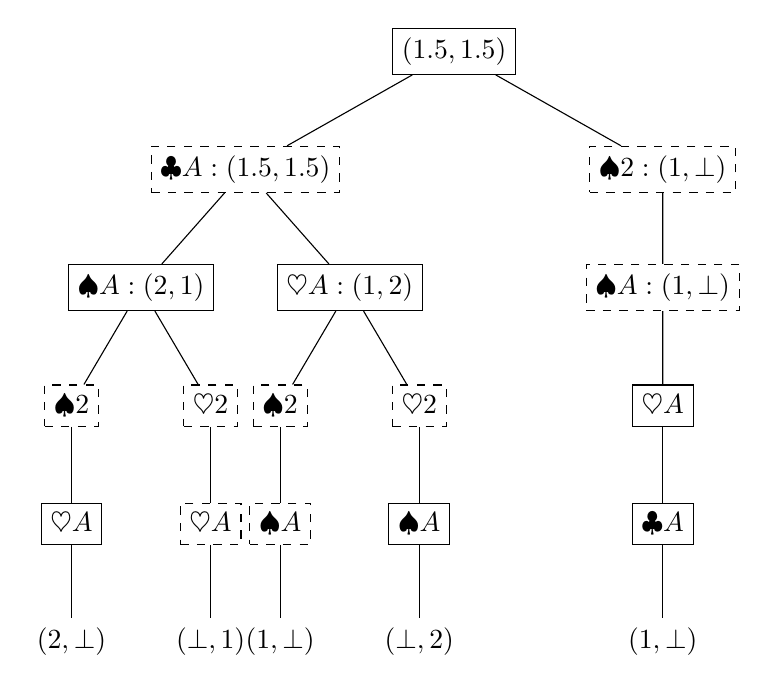
\begin{tikzpicture}[level/.style={sibling distance=53mm/#1}, scale=1]
    \node [draw] {$(1.5,1.5)$}
        child {node [draw, dashed]  {$\clubsuit A: (1.5,1.5)$}
            child {node [draw] {$\spadesuit A: (2,1)$}
                child {node [draw, dashed] {$\spadesuit 2$}
                    child {node [draw] {$\heartsuit A$}
                        child {node {$(2,\bot)$}}}}
                child {node [draw, dashed] {$\heartsuit 2$}
                    child {node [draw, dashed] {$\heartsuit A$}
                        child {node {$(\bot, 1)$}}}}}
            child {node [draw] {$\heartsuit A: (1,2)$}
                child {node [draw, dashed] {$\spadesuit 2$}
                    child {node [draw, dashed] {$\spadesuit A$}
                        child {node {$(1,\bot)$}}}}
                child {node [draw, dashed] {$\heartsuit 2$}
                    child {node [draw] {$\spadesuit A$}
                        child {node {$(\bot,2)$}}}}}}
        child {node [draw, dashed]  {$\spadesuit 2: (1,\bot)$}
            child {node [draw, dashed] {$\spadesuit A: (1,\bot)$}
                child {node [draw] {$\heartsuit A$}
                    child {node [draw] {$\clubsuit A$}
                        child {node {$(1,\bot)$}}}}}}
    ;
    \end{tikzpicture}
\end{figure}


In practice, taking any set $W$ won't work to have this system of subsets of possible worlds. To have a correct number of worlds for each hand of each player, we need to have similarities between the worlds of $W$. To do this, we use a small set of initial worlds and we create the set $W$ by taking all the possible permutations of the hands with this initial set. So in Alg. \ref{algo:perm} $\mbox{\em generateWorlds}$ samples some worlds and then returns all the permutations of those worlds. $max_i$ follows the scheme explained before. $\mbox{\em criterion}_i$ selects the value with the best average score over the possible worlds of $i$. We prune if all the scores of one value are worse than another one.

\begin{algorithm}
\caption{Fusion}
\label{algo:perm}
\begin{algorithmic}
\Function{$\mbox{\em max}_i$}{$a$, $b$}
%    \State $r \gets {\bf 0} \in \mathbb{R}^{|\mbox{\em \tiny legal}(h,s)|}$
%    \State $r \in \mathcal{V}$
    \For{$h$ possible hand of $i$}
        \State $\mbox{\em score}_a \gets \sum_{w \in P_h}a_w$
        \State $\mbox{\em score}_b \gets \sum_{w \in P_h}b_w$
        \If {$\mbox{\em score}_a < \mbox{\em score}_b$}
            \For{$w \in P_h$}
                \If{Max team} $r_w \gets b_w$
                {\emph else}
                     $r_w \gets a_w$
                \EndIf
            \EndFor
        \Else
            \For{$w \in P_h$}
                \If{Max team}
                 $r_k \gets a_w$
                {\bf else}
                 $r_k \gets b_w$
                \EndIf
            \EndFor
        \EndIf
    \EndFor
    \State \Return r
\EndFunction
\end{algorithmic}
\end{algorithm}


\section{Implementation}

For the implementation, we have adapted the above formalization to the code. This allows us to keep some flexibility in the rules used later. We put the organization of the card game into one file. This file is for the general game, and when rule-dependent functions are needed, we call them in the specific rule file associated with them.

A simple modification in the Makefile selects which game is played and which rule file is read when these rule-dependent functions are used. It uses a game class that stores the information about the game being played: the contract, the cards already played, who has to play, the scores of the teams, what the current trick consists of, and who is the leader of that trick. We have a \emph{player} class, which contains the information that a player has (his hand, what he knows about the other hands, etc). The communication with the player is realized in the methods of this class. The selection of the card to play is implemented by a function pointer, which is an attribute of the player class. Several functions have been created to select a card. We define this attribute of the player class to define its strategy. 

We have collected all these different strategies in a directory. These are mainly the strategies described above. Since they often follow the same pattern, as we have explained, we used the algorithm of Figure \ref{algo:template}. We then used an abstract class for each tree strategy. This abstract class is then specified into precise classes corresponding to each strategy that follows the template. In each class, the specification-dependent functions, such as $\max_i$, are implemented as attributes. To invoke the function that selects a card, we call the template with the class of the selected specification. 

To encode the knowledge, the player class has an attribute $\mbox{\em have\_not}$, which is an array containing the cards that this player knows that the other players do not have. This knowledge is used to generate the worlds used in the strategy functions, so that the generated worlds respect what the player knows about the others. 

As for the basic types, we used bit vectors (mainly a set of unsigned integers) to represent the set of cards. For example, in Belote with its 32 cards, we used one unsigned integer. If a bit in a representing vector is set to true, then the corresponding card in the deck is contained in the set. 

You can start the games by choosing which hands are played, which strategies are used by each player, and how many games are played. We ran several experiments with this structure. 

\section{Experiments}

%We adapted the formalization of Section \ref{section:formalisation}. 
We tested the approach in two different games: Belote and Bridge. 
%Other games are to be implemented like Skat and maybe Tarot. 
While Bridge is well-studied, our core interest is in (La) Belote, a French national card game for four players. %\footnote{\url{https://en.wikipedia.org/wiki/Belote}}. 
%
For the player's strategy we implemented the three algorithms we discussed and a random card strategy, to have some kind of naive player. We then compared pairs of algorithms. In both cases there are two teams, so we assigned one strategy to one team and the other to the second team. We played matches of 100 different deal (same across the different experiments). With each deal, we play once as it is, and then swap the team's positions, so that it is fair. We measure the score made by the team of the first player to play. In each experiment we finally collect the 200 scores across these games. We add the 100 scores made by one strategy, and the 100 scores made by the other, and deduce the percentage of the total amount of points per game that on strategy wins over the other. 

In each algorithm there are some hyperparameters to fix: $n_{\mbox{\em \tiny sample}}$ is the number of worlds used in the algorithm. $\mbox{\em depth-leaf}$ in $\alpha\mu$ and the fusion algorithm is the depth at which we stopped the specification to end the tree with PIMC (this is done for complexity issues, it is also done in \cite{cazenave_$$alpha$$_2021}. $\mbox{\em depth-rd}$ is the depth at which pimc is stopped to end the tree with the an average of the random playouts. 

%We derived a formula that allows us to estimate the approximation made. 
For Belote, we derived a $10\%$ approximation of the score, that was valid with $95\%$ probability with these random playouts. For Bridge, we imposed a low value of $\mbox{\em depth-rd}$ for matters of complexity, and the bounds on the approximation made were not consistent. We tried to keep the same hyperparameters for all the algorithms, but Fusion needed more worlds than the others.
%so there is an asymmetry (this is a mistake that could be easily fixed with time to do again the experiments). 
%$x\frac{\sum_0 scores - \sum_1 scores}{100 \times TotalPoints}
%
%
\begin{figure}[t]
    \centering
    \label{fig:exp-be}
\vspace{-0.2cm}    
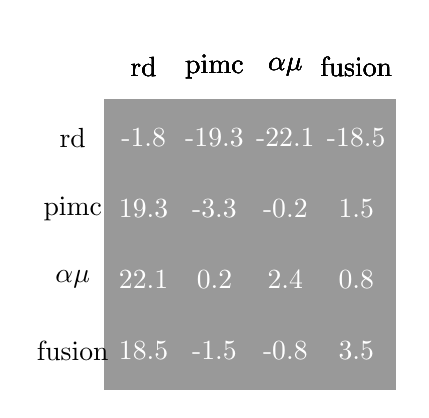
\begin{tikzpicture}[scale=0.9]
  \foreach \y [count=\n] in {
      {-1.8,-19.3,-22.1,-18.5},
      {19.3,-3.3,-0.2,1.5},
      {22.1,0.2,2.4,0.8},
      {18.5,-1.5,-0.8,3.5},
    } {
      % column labels
    \node[minimum size=10mm] at (1, 0) {rd};
    \node[minimum size=10mm] at (2, 0) {pimc};
    \node[minimum size=10mm] at (3, 0) {$\alpha\mu$};
    \node[minimum size=10mm] at (4, 0) {fusion};
      % heatmap tiles
      \foreach \x [count=\m] in \y {
        \node[fill=black!40!white, minimum size=10mm, text=white] at (\m,-\n) {\x};
      }
    }

  % row labels
  \foreach \a [count=\i] in {rd,pimc,$\alpha\mu$,fusion} {
    \node[minimum size=10mm] at (0,-\i) {\a};
  }
\end{tikzpicture}
    \caption{Belote; team 0 in rows, team 1 in columns. Pimc: $n_{\mbox{\em \tiny sample}} = 10$. $\alpha\mu$: $n_{\mbox{\em \tiny sample}} = 10$, $\mbox{\em depth-leaf} = 5$, $\mbox{\em depth-rd} = 20$. Fusion: $n_{\mbox{\em \tiny sample}} = 24$, $\mbox{\em depth-leaf} = 5$, $\mbox{\em depth-rd} = 20$.}
\end{figure}
%
\begin{figure}[t]
\label{fig:exp-br}
    \centering
\vspace{-0.7cm}      
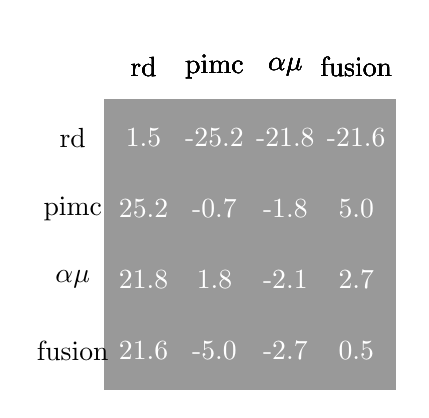
\begin{tikzpicture}[scale=0.9]
  \foreach \y [count=\n] in {
      {1.5,-25.2,-21.8, -21.6},
      {25.2,-0.7,-1.8, 5.0},
      {21.8,1.8,-2.1, 2.7},
      {21.6,-5.0,-2.7,0.5},    } {
      % column labels
    \node[minimum size=10mm] at (1, 0) {rd};
    \node[minimum size=10mm] at (2, 0) {pimc};
    \node[minimum size=10mm] at (3, 0) {$\alpha\mu$};
    \node[minimum size=10mm] at (4, 0) {fusion};
      % heatmap tiles
      \foreach \x [count=\m] in \y {
        \node[fill=black!40!white, minimum size=10mm, text=white] at (\m,-\n) {\x};
      }
    }

  % row labels
  \foreach \a [count=\i] in {rd,pimc,$\alpha\mu$,fusion} {
    \node[minimum size=10mm] at (0,-\i) {\a};
  }
\end{tikzpicture}
    \caption{Bridge; team 0 in rows, team 1 in columns. Pimc: $n_{\mbox{\em \tiny sample}} = 10$. $\alpha\mu$: $n_{\mbox{\em \tiny sample}}$, $\mbox{\em depth-leaf} = 5$, $\mbox{\em depth-rd} = 9$, Fusion: $n_{\mbox{\em \tiny sample}} = 24$, $\mbox{\em depth-leaf} = 5$, $\mbox{\em depth-rd} = 20$.}
\end{figure}
% 
%
%We can see %in \ref{fig:exp-be} and \ref{fig:exp-br} 
%that 
%
All algorithms are better than random. We can also see that the $\alpha\mu$ algorithm is slightly better than the others. Let us note that all these algorithms are designed to play against smart players so the differences of the scores against random are not significant (PIMC being better than $\alpha\mu$ in beating random in Bridge is not relevant). Fusion algorithm is slightly worse than the others. However, pruning in the Fusion algorithm needs to be improved. 

In Belote vs.\ another AI PIMC ($n_{\mbox{\em \tiny sample}}=10$, $\mbox{\em depth-rd} = 25$) we
%the result are that over the same 100 games the player achieved 8399 points as 
%a declarer, while the competitor achieved 6823 as a declarer 
%leading 
found a $9.7\%$ gain in the max.\ score on average. 
%Games played in a textual interface indicated Human-adequate play of our AI.


\section{Conclusion}

We presented an efficient framework for imperfect information card games and found a factorization of the search in a template that captures the main ingredients of the search. We then analyzed three different algorithms and derived the impact of the information given during the algorithm on the decisions it makes. Finally, we designed a new algorithm that tries to respect known information more. We also estimated the effects of truncating the search tree with random rollouts, and the information gain obtained by $\alpha\mu$.
% 
To continue this work, we need to explore more deeply the possibilities for a better pruning of the tree. 
%We also need to conduct a wider set experiments with new games and new %algorithms, especially to compete with existing algorithms %\cite{edelkamp_knowledge-based_2021}
Last, but not least we will aim at card games with \emph{talon} 
%like Rummy, Mahjong, or Canasta 
that do not yet fit the setting.


\section{Acknowledgments}

This research was partly funded by AFOSR project Flexible and Resilient Auton. Systems (FRAS) and by the Czech Science Foundation, grant number 22-30043S.
%
% ---- Bibliography ----
%
% BibTeX users should specify bibliography style 'splncs04'.
% References will then be sorted and formatted in the correct style.
%
% \bibliographystyle{splncs04}
% \bibliography{mybibliography}
%
\begin{thebibliography}{8}

    \bibitem{connectfour}
    L. V. Allis: A knowledge-based approach to connect-four. The game is solved: White wins. Master's Thesis, Vrije Univeriteit, The Netherlands (1998).

    \bibitem{Oware}
    Xavier Blanvillain: Oware is Strongly Solved. In: Computers and Games, Springer (2022).

    \bibitem{poker}
    Michael Bowling, Neil Burch, Michael Johanson, Oskari Tammelin: Heads-up limit hold'em poker is solved. Commun. ACM, 60(11), 81-88 (2017).

    \bibitem{calculating_pimc}
    Alan Brennan, Samer Kharroubi, Anthony O'Hagan, Jim Chilcott: Calculating Partial Expected Value of Perfect Information via Monte Carlo Sampling Algorithms. Medical Decision Making, 27(4), 448-470 (2007).

    \bibitem{DBLP:conf/ijcai/BuroLFS09}
    M. Buro, J. R. Long, T. Furtak, and N. R. Sturtevant. Improving state evaluation, inference, and search in trick-based card games. IJCAI, p 1407–1413, 2009.

    \bibitem{DBLP:journals/corr/abs-1911-07960}
    Tristan Cazenave, Véronique Ventos: The $\alpha\mu$ Search Algorithm for the Game of Bridge. (2019).

    \bibitem{cazenave_$$alpha$$_2021}
    Tristan Cazenave, Véronique Ventos: The $\alpha\mu$ Search Algorithm for the Game of Bridge. Communications in Computer and Information Science, Springer, 1-16 (2021).

    \bibitem{DBLP:conf/ecai/CohensiusMOS20}
    G. Cohensius, R. Meir, N. Oved, and R. Stern. Bidding in spades. In ECAI, pages 387–394, 2020.

    \bibitem{edelkamp_challenging_2019}
    Stefan Edelkamp: Challenging Human Supremacy in Skat. Proceedings of the Twelfth International Symposium on Combinatorial Search (SOCS) 2019, 52-60.

    \bibitem{edelkamp_knowledge-based_2021}
    Stefan Edelkamp: Knowledge-Based Paranoia Search in Trick-Taking. CoRR, abs/2104.05423 (2021).

    \bibitem{hope}
    S. Edelkamp. Improving computer play in Skat with hope cards. (2023).

    \bibitem{finnsson2007cadia}
    H. Finnsson. Cadia-player: A general game playing agent. PhD thesis, 2007.

    \bibitem{frank1998search}
    I. Frank and D. Basin. Search in games with incomplete information: A case study using bridge card play. Artificial Intelligence, 100(1-2):87–123, 1998

    \bibitem{ninemenmorris}
    R. Gasser: Harnessing Computational Resources for Efficient Exhaustive Search. PhD Thesis, ETH Zürich (1995).

    \bibitem{GIB}
    M. Ginsberg: Step toward an expert-level Bridge-playing program. In: IJCAI, 584-589 (1999).

    \bibitem{knuth_analysis_1975}
    Donald E. Knuth, Ronald W. Moore: An analysis of alpha-beta pruning. Artificial Intelligence, 6(4), 293-326 (1975).

    \bibitem{diplomkupfersc}
    Sebastian Kupferschmid: Entwicklung eines Double-Dummy Skat Solvers mit einer Anwendung für verdeckte Skatspiele. Master's Thesis, University of Freiburg (2006).

    \bibitem{ab_generalisation_2022}
    Junkang Li, Bruno Zanuttini, Tristan Cazenave, Véronique Ventos: Generalisation of alpha-beta search for AND-OR graphs with partially ordered values. Research Report, GREYC CNRS UMR 6072, Universite de Caen (May 2022).

    \bibitem{understanding_pimc}
    Jeffrey Richard Long, Nathan R Sturtevant, Michael Buro, Timothy Furtak: Understanding the success of perfect information monte carlo sampling in game tree search. Twenty-Fourth AAAI Conference on Artificial Intelligence (2010).

    \bibitem{DBLP:journals/corr/MoravcikSBLMBDW17}
    Matej Moravčík, Martin Schmid, Neil Burch, Viliam Lisý, Dustin Morrill, Nolan Bard, Trevor Davis, Kevin Waugh, Michael Johanson, Michael H. Bowling: DeepStack: Expert-Level Artificial Intelligence in No-Limit Poker. CoRR, abs/1701.01724 (2017).

    \bibitem{Perolat_2022}
    J. Perolat, B. D. Vylder, D. Hennes, E. Tarassov, F. Strub, V. de Boer, P. Muller, J. T. Connor, N. Burch, T. Anthony, S. McAleer, R. Elie, S. H. Cen, Z. Wang, A. Gruslys, A. Malysheva, M. Khan, S. Ozair, F. Timbers, T. Pohlen, T. Eccles, M. Rowland, M. Lanctot, J.B. Lespiau, B. Piot, S. Omidshafiei, E. Lockhart, L. Sifre, N. Beauguerlange, R. Munos, D. Silver, S. Singh, D. Hassabis, and K. Tuyls. Mastering the game of stratego with model free multiagent reinforcement learning. Science, 378(6623):990–996, dec 2022.

    \bibitem{DBLP:journals/computer/RomeinB03}
    John W. Romein, Henri E. Bal: Solving Awari with Parallel Retrograde Analysis. Computer, 36(10), 26-33 (2003).

    \bibitem{checkers}
    Jonathan Schaeffer, Yngvi Björnsson, N. Burch, Akihiro Kishimoto, Martin Müller, Robert Lake, Paul Lu, Steve Sutphen: Solving Checkers. In: IJCAI, 292-297 (2005).

    \bibitem{Schiffel2011a}
    S. Schiffel and M. Thielscher. Reasoning about general games described in gdl-ii. In Proceedings of the AAAI Conference on Artificial Intelligence, pages 846–851. AAAI Press, 2011.

    \bibitem{AlphaGo}
    D. Silver and A. H. et al. Mastering the game of Go with deep neural networks and tree search. Nature, 529:484, 2016.

    \bibitem{alphazero}
    David Silver, Thomas Hubert, Julian Schrittwieser, Ioannis Antonoglou, Matthew Lai, Arthur Guez, Marc Lanctot, Laurent Sifre, Dharshan Kumaran, Thore Graepel, Timothy Lillicrap, Karen Simonyan, Demis Hassabis: Mastering Chess and Shogi by Self-Play with a General Reinforcement Learning Algorithm. Tech Report, arxiv, 1712.018 (2017).

    \bibitem{multi-pruning}
    N. R. Sturtevant and R. E. Korf. On pruning techniques for multi-player games. AAAI/IAAI, 49:201–207, 2000.

    \bibitem{DBLP:conf/cg/SturtevantW06}
    Nathan R. Sturtevant, Adam M. White: Feature Construction for Reinforcement Learning in Hearts. In: Computers and Games, Springer, 122-134 (2006).

\end{thebibliography}
\end{document}


    